%%%%%%%%%%%%%%%%%%%%%%%%%%%%%%%%%%%%%%%%%
% kaobook
% LaTeX Template
% Version 1.3 (18/2/20)
%
% This template originates from:
% https://www.LaTeXTemplates.com
%
% For the latest template development version and to make contributions:
% https://github.com/fmarotta/kaobook
%
% Authors:
% Federico Marotta (federicomarotta@mail.com)
% Giuseppe Silano (g.silano89@gmail.com)
% Based on the doctoral thesis of Ken Arroyo Ohori (https://3d.bk.tudelft.nl/ken/en)
% and on the Tufte-LaTeX class.
% Modified for LaTeX Templates by Vel (vel@latextemplates.com)
%
% License:
% CC0 1.0 Universal (see included MANIFEST.md file)
%
%%%%%%%%%%%%%%%%%%%%%%%%%%%%%%%%%%%%%%%%%

%----------------------------------------------------------------------------------------
%	PACKAGES AND OTHER DOCUMENT CONFIGURATIONS
%----------------------------------------------------------------------------------------

\documentclass[
	fontsize=10pt, % Base font size
	twoside=true, % Use different layouts for even and odd pages (in particular, if twoside=true, the margin column will be always on the outside)
	%open=any, % If twoside=true, uncomment this to force new chapters to start on any page, not only on right (odd) pages
	secnumdepth=1, % How deep to number headings. Defaults to 1 (sections)
	%chapterprefix=true, % Uncomment to use the word "Chapter" before chapter numbers everywhere they appear
	%chapterentrydots=true, % Uncomment to output dots from the chapter name to the page number in the table of contents
	numbers=noenddot, % Comment to output dots after chapter numbers; the most common values for this option are: enddot, noenddot and auto (see the KOMAScript documentation for an in-depth explanation)
	%draft=true, % If uncommented, rulers will be added in the header and footer
	%overfullrule=true, % If uncommented, overly long lines will be marked by a black box; useful for correcting spacing problems
]{kaobook}

% Choose the language
\usepackage[english]{babel} % Load characters and hyphenation
\usepackage[english=british]{csquotes}	% English quotes

% Load packages for testing
\usepackage{blindtext}
%\usepackage{showframe} % Uncomment to show boxes around the text area, margin, header and footer
%\usepackage{showlabels} % Uncomment to output the content of \label commands to the document where they are used

% Load the bibliography package
\usepackage{styles/kaobiblio}
\addbibresource{book-template.bib} % Bibliography file

% Load mathematical packages for theorems and related environments. NOTE: choose only one between 'mdftheorems' and 'plaintheorems'.
\usepackage{styles/mdftheorems}
%\usepackage{styles/plaintheorems}

% Load the package for hyperreferences
\usepackage{styles/kaorefs}

\graphicspath{{images/}{./}} % Paths in which to look for images

\makeindex[columns=3, title=Alphabetical Index, intoc] % Make LaTeX produce the files required to compile the index

\makeglossaries % Make LaTeX produce the files required to compile the glossary

\makenomenclature % Make LaTeX produce the files required to compile the nomenclature

%----------------------------------------------------------------------------------------

\begin{document}

%----------------------------------------------------------------------------------------
%	BOOK INFORMATION
%----------------------------------------------------------------------------------------

\titlehead{Preliminary draft}
% \subject{Subject}

\title[Calculus Ia]{Calculus Ia: Limits and differentiation}
% \subtitle{Subtitle}

\author[Yichao]{Yichao Huang}

\date{\today}

\publishers{University of Helsinki}

%----------------------------------------------------------------------------------------

\frontmatter % Denotes the start of the pre-document content, uses roman numerals

%----------------------------------------------------------------------------------------
%	OPENING PAGE
%----------------------------------------------------------------------------------------

% \makeatletter
% \extratitle{
% 	% In the title page, the title is vspaced by 9.5\baselineskip
% 	\vspace*{9\baselineskip}
% 	\vspace*{\parskip}
% 	\begin{center}
% 		% In the title page, \huge is set after the komafont for title
% 		\usekomafont{title}\huge\@title
% 	\end{center}
% }
% \makeatother

%----------------------------------------------------------------------------------------
%	COPYRIGHT PAGE
%----------------------------------------------------------------------------------------

\makeatletter
\uppertitleback{\@titlehead} % Header

\lowertitleback{
	\textbf{Disclaimer} \\
	Any errors that remain are the author's sole responsibility.
	
	\medskip
	
	\textbf{No copyright} \\
	\cczero\ This book is released into the public domain using the CC0 code. To the extent possible under law, I waive all copyright and related or neighbouring rights to this work.
	
	To view a copy of the CC0 code, visit: \\\url{http://creativecommons.org/publicdomain/zero/1.0/}
	
	\medskip
	
	\textbf{Colophon} \\
	This document was typeset with the help of \href{https://sourceforge.net/projects/koma-script/}{\KOMAScript} and \href{https://www.latex-project.org/}{\LaTeX} using the \href{https://github.com/fmarotta/kaobook/}{kaobook} class.
	
	\medskip
	
	\textbf{Publisher} \\
	First printed in Fall 2020 by \@publishers
}
\makeatother

%----------------------------------------------------------------------------------------
%	DEDICATION
%----------------------------------------------------------------------------------------

\dedication{
	\textbf{Don't just read it; fight it!} Ask your own question, look for your own examples, discover your own proofs. Is the hypothesis necessary? Is the converse true? What happens in the classical special case? What about the degenerate cases? Where does the proof use the hypothesis?\\
	\flushright -- Paul Halmos
}

%----------------------------------------------------------------------------------------
%	OUTPUT TITLE PAGE AND PREVIOUS
%----------------------------------------------------------------------------------------

% Note that \maketitle outputs the pages before here

% If twoside=false, \uppertitleback and \lowertitleback are not printed
% To overcome this issue, we set twoside=semi just before printing the title pages, and set it back to false just after the title pages
\KOMAoptions{twoside=semi}
\maketitle
\KOMAoptions{twoside=false}

%----------------------------------------------------------------------------------------
%	PREFACE
%----------------------------------------------------------------------------------------

\chapter*{Preface}

This lecture note is as boring as it gets, since it tries to be politically correct and does not contain:
\begin{enumerate}
	\item Your own effort in trying new things in mathematics;
	\item Your own taste of what is beautiful and what is not;
	\item Your happiness in understanding a concept or finding a proof;
	\item Your failures and experiences to refine your future choices;
	\item Your interaction and teamwork with your friends;
	\item Your lunch hours, roadtrips, family, dreams, and drunken moments (some by alcohol, some by art, some by people);
	\item Your splendid life with all the possibilities ahead.
\end{enumerate}
The goal of this lecture note is to simply provide some remainders in case one needs them. Like a photo album. In some sense, the primary goal would be for you to understand some mathematical concepts, and gradually you should be able to express your ideas in mathematical terms with ease.

It is often asked about a reference book for this course. I don't want to recommend anything in particular, but I would recommend to have at least one ``classical'' textbook at hand, preferably with detailed solutions to the exercises. Try the exercise yourself first, and when you really get stuck, read the solution, then try the exercise again several days later.

Instead I could recommand some ``casual'' books:
\begin{enumerate}
	\item <<Gödel, Escher, Bach: An Eternal Golden Braid>>, Hofstadter, Basic Books.
	\item <<Proofs from THE BOOK>>, Aigner-Ziegler, Springer.\sidenote{This one is not that casual\dots !}
	\item <<How to solve it>>, Pólya, Princeton University Press.
	\item <<Flatland: A Romance of Many Dimensions>>, Abbott, Seeley \& Co.
\end{enumerate}

\begin{flushright}
Have fun!

Yichao Huang
\end{flushright}

P.S. Although this note can be publicly distributed and reused, it is not my intention. It thus contains many personal touches and certainly does not stand the test of time.

%----------------------------------------------------------------------------------------
%	TABLE OF CONTENTS & LIST OF FIGURES/TABLES
%----------------------------------------------------------------------------------------

\begingroup % Local scope for the following commands

% Define the style for the TOC, LOF, and LOT
%\setstretch{1} % Uncomment to modify line spacing in the ToC
%\hypersetup{linkcolor=blue} % Uncomment to set the colour of links in the ToC
\setlength{\textheight}{23cm} % Manually adjust the height of the ToC pages

% Turn on compatibility mode for the etoc package
\etocstandarddisplaystyle % "toc display" as if etoc was not loaded
\etocstandardlines % "toc lines as if etoc was not loaded

\tableofcontents % Output the table of contents

\listoffigures % Output the list of figures

% Comment both of the following lines to have the LOF and the LOT on different pages
\let\cleardoublepage\bigskip
\let\clearpage\bigskip

% \listoftables % Output the list of tables

\endgroup

%----------------------------------------------------------------------------------------
%	MAIN BODY
%----------------------------------------------------------------------------------------

\mainmatter % Denotes the start of the main document content, resets page numbering and uses arabic numbers
\setchapterstyle{kao} % Choose the default chapter heading style
\chapter{A ``gentle'' introduction to the language of mathematics}

Since this notes is written during the Corona time, let us start by reviewing some common misunderstandings.

Do the following sentences convey the same message?\sidenote{Does ``The government now recommands wearing masks'' implies ``The government recommanded against wearing masks before''?}
\begin{enumerate}
	\item The government has no recommandation for wearing masks.
	\item The government does not recommand wearing masks.
	\item The government recommand against wearing masks.
\end{enumerate}

\section{Mathematical symbols}
Some symbols are specific to mathematics, such as
\begin{equation*}
\begin{split}
\forall&\quad \text{for all}\\
\exists&\quad \text{there exist(s)}\\
\lor&\quad \text{or}\\
\land&\quad \text{and}\\
\infty&\quad \text{infinity}
\end{split}
\end{equation*}
and many more.\sidenote{In short, this course BSMA1002 is about the symbol $'$ and the next course BSMA1003 is about the symbol $\int$.}

One uses these symbols to write statements in mathematics. For example, one can write
\begin{equation*}
\forall x\in\mathbb{R}, (x^2-1\geq 0)\lor (x^3+1\geq 0).
\end{equation*}
This reads (from left to right!) ``for all real number $x$, (we have) $x^2-1\geq 0$ or $x^3+1\geq 0$''. In practice, the symbol $\lor$ is not that often used, and one encounters more often
\begin{equation*}
\forall x\in\mathbb{R}, (x^2-1\geq 0)~\text{or}~(x^3+1\geq 0).
\end{equation*}
Notice that the meaning of the word ``or'' is inexclusive.\sidenote{\textbf{Exclusive or} or \textbf{exclusive disjunction} is a logical operation that outputs true only when inputs differ (one is true, the other is false). In logic, \textbf{or} by itself means the \textbf{inclusive or}, distinguished from an exclusive or, which is false when both of its arguments are true, while an "or" is true in that case. In sum, $A\lor B$ is true if $A$ is true, or if $B$ is true, or if both $A$ and $B$ are true.} Also, notice that this phrase is not true, but that is not the point here.

One can ``operate'' on statements. For example, with the \textbf{negation} symbol
\begin{equation*}
\neg\quad \text{not}
\end{equation*}
one can ``negate'' a statement:
\begin{equation*}
\neg \left(\forall x\in\mathbb{R}, (x^2-1\geq 0)~\text{or}~(x^3+1\geq 0)\right).
\end{equation*}
What does it mean? How do one write it in plain language?

(Before moving on, one could first to come up with a personal attempt. The goal is not to succeed at the first try, but to, \emph{inter alia}, figure out some patterns and be aware of the possible difficulties.)

The general rule for negating a statement is the following: (tbc).\sidenote{Don't try to remember these sentences, but rather, do some examples and \textbf{understand the principle behind it}.}

For the example above, an equivalent way of writing the statement
\begin{equation*}
\neg \left(\forall x\in\mathbb{R}, (x^2-1\geq 0)~\text{or}~(x^3+1\geq 0)\right)
\end{equation*}
is
\begin{equation*}
\exists x\in\mathbb{R}, \neg(x^2-1\geq 0)~\text{and}~\neg(x^3+1\geq 0).
\end{equation*}
And if we really want to get rid of the negation symbol, we can also write it as
\begin{equation*}
\exists x\in\mathbb{R}, (x^2-1<0)~\text{and}~(x^3+1<0).
\end{equation*}

\begin{remark}
In practice, this means that if $P$ is some property and if one wants to \textbf{disprove} a statement of type  ``for all $x$, $P$ is true'' ($\forall x, P$), one should show the existence of some $x$ such that $P$ is false ($\exists x, \neg P$). Showing that such $x$ exists can be done by explicit construction (``pulling a rabbit out of a hat''), or by abstraction (without necessarily knowing all the properties of such $x$).
\end{remark}

\textbf{Implications} are highly frequent statements in mathematics.\sidenote{Which phrase is an implication in the classical \textbf{syllogism} ``All men are mortal. Socrates is a man. Therefore, Socrates is mortal.''?} If $P$ and $Q$ are two properties (or two statements), the symbol\sidenote{In some Finnish textbooks it is written $\rightarrow$. Different people use different notations, but usually they look similar and understandable by context.}
\begin{equation*}
\Rightarrow\quad\text{implies}
\end{equation*}
used in the following statement
\begin{equation*}
P\Rightarrow Q
\end{equation*}
means ``If $P$ is true, then $Q$ is true''. It does not give information on $Q$ if $P$ is false.

One can draw a \textbf{truth table} to understand better the symbol $\Rightarrow$. In the table, $1$ means ``true'' and $0$ means ``false'', and I leave you to figure out the rest.

(tbc)

It is quite useful to realize that the implication symbol can be replaced by other symbols before. At first sight this mights seem strange, but let us draw the table of truth for
\begin{equation*}
(\neg P) \lor Q
\end{equation*}
and compare it to the table before:

(tbc)

\textbf{Equivalence} of two statements $P$ and $Q$, with the symbol
\begin{equation*}
P\equiv Q
\end{equation*}
should be understood as two implications:
\begin{equation*}
P\Rightarrow Q\quad\text{and} Q\Rightarrow P.
\end{equation*}
It simply says that they are either both true or both false.\sidenote{Try to draw the truth table (on a paper, on an electronic device or in your head)!}

\begin{proposition}
The following statements are equivalent:\sidenote{Personal dedication to my undergrad teacher Mr. Mohan: ``LASSE'' (Les assertions suivantes sont équivalentes).}
\begin{enumerate}
	\item \begin{equation*}P\Rightarrow Q.\end{equation*}
	\item \begin{equation*}(\neg P) \lor Q.\end{equation*}
\end{enumerate}
\end{proposition}

\begin{proposition}
The following statements are equivalent:\sidenote{So, what does ``$((\neg P) \lor Q)\land((\neg Q) \lor P)$'' mean?}
\begin{enumerate}
	\item \begin{equation*}P\equiv Q.\end{equation*}
	\item \begin{equation*}(P\Rightarrow Q)\land(Q\Rightarrow P).\end{equation*}
\end{enumerate}
It is a little self-referencing if you take it as the definition of equivalence!
\end{proposition}

\textbf{Proof by contradiction} is also commonly used in mathematics (and in everyday life).\sidenote{Proof by contradiction is formulated as $P\equiv P\lor \bot\equiv \neg(\neg P)\lor \bot\equiv \neg P\to\bot$, where $\bot$ is a logical contradiction or a false statement (a statement which true value is false). If $\bot$ is reached via $\neg P$ via a valid logic, then $\neg P\to \bot$ is proved as true so $P$ is proved as true. I didn't bother to read the above phrases myself (I copied it from \href{https://en.wikipedia.org/wiki/Proof_by_contradiction}{Wikipedia}), since in practice, one should seize the \textbf{idea} (which I think you all have it naturally) rather than relying on formal manipulation of symbols. It is up to you to find out what is the best way to understand a new concept!} The principle can be summarized as the following: (tbc)

\begin{figure}[h]
  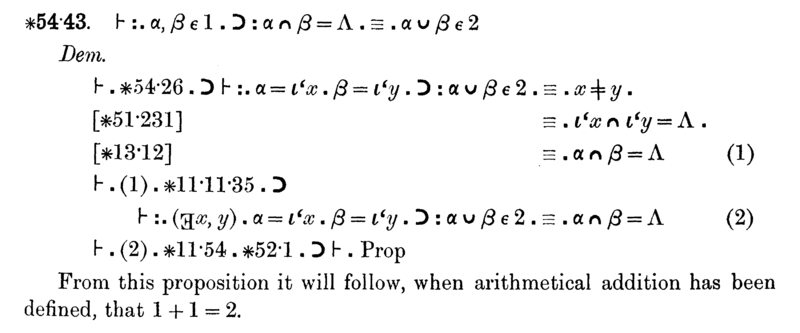
\includegraphics{Principia_Mathematica.png}
  \caption{Whitehead and Russell proving $1+1=2$. Full story \href{https://en.wikipedia.org/wiki/Principia_Mathematica}{here}.}
  \label{fig:PrincipiaMathematica}
\end{figure}

\begin{remark}
Of course, mathematicians (or scientists) never write with symbols only, unless you are a hardcore logician. You will soon know where to draw the line: the above is just a showcase of the mathematical rigor.
\end{remark}

One of the advantages of mathematics compared to other science, is that (almost) all proofs are reproducible and can be checked.\sidenote{Even \href{https://www.quantamagazine.org/titans-of-mathematics-clash-over-epic-proof-of-abc-conjecture-20180920/}{this one}.} It is a good way to train your critical thinking skills: by doing mathematics (the right way!), you are living one of the rare moments where you can distinguish completely right from wrong and form a clear judgement.

\section{Mathematical induction}
One of the early difficulties of transitioning into a good undergrad student is to write mathematical sound and concise proofs. We have already seen what is proof by contradiction; let us review another classical proof technique: \textbf{proof by induction}.

Here is a learning technique: you can \textbf{start by an example before reading the theoretical descriptions}. So let us search ``proof by induction'' on the internet, go to the Wikipedia page, and check out the following example:

\begin{example}[Sum of consecutive natural numbers]
\dots
\end{example}

\pagelayout{wide} % No margins
\addpart{[Week I]\\What are\dots sets?}
\pagelayout{margin} % Restore margins

\chapter{Sets: definitions and properties}

\section{Sets, elements, subsets}

\section{Union, intersection, cardinality}

\section{Finite sets and a taste of combinatorics}

\section{Story time: some paradoxes}

(tbc)

For a more elaborated logic paradox of the same flavor, check out the poem on the door of Åsa Hirvonen (last retrieved: August 2020).

\chapter{Infimum and supremum}
``In mathematics, a small positive infinitesimal quantity, usually denoted $\epsilon$, whose limit is usually taken as $\epsilon\to 0$.''

\begin{flushright}
-- Wolfram \href{https://mathworld.wolfram.com/Epsilon.html}{MathWorld}.
\end{flushright}

All symbols are created equal, but some symbols are more equal than others. You can write $y=f(x)$ or $b=f(a)$ or $v=f(u)$ or $s=f(t)$, but at least in this course, we reserve the notation $\epsilon$ (and later $\delta$) for special purposes.

\section{Relations and ordering}
\dots

\section{An epsilon of room}

\section{Development: the Archimedean property}

\pagelayout{wide} % No margins
\addpart{[Week II]\\What are\dots sequences?}
\pagelayout{margin} % Restore margins

\chapter{Sequences: definitions and properties}

\section{Classical sequences}

\section{Limit of a sequence}

\section{Squeeze theorem}

\section{Indeterminate forms}

\section{Development: Bolzano-Weierstrass theorem}

\pagelayout{wide} % No margins
\addpart{[Week III\&IV]\\What are\dots functions?}
\pagelayout{margin} % Restore margins

\chapter{Functions: definitions and properties}
In high school, most functions are given in the form of a formula:
\begin{equation*}
y=f(x)=x^{2}+1.
\end{equation*}

However, in full generality, a function is defined in a more abstract way. The essential idea is to associate an element to a given element (in the example above, for each real number $x$, we associate the real number $y=x^2+1$). The abstract definition has many advantages and covers more situations, for example, we will see that a sequence can be seen as a function (from a set of integers $\mathbb{Z}_{n\geq 0}$ to the set of real numbers $\mathbb{R}$).

\section{Notations}

(tbc)

Sometimes, by abuse of notation,\sidenote{Sometimes it means ``The author is tired.''}

\begin{example}
The Möbius function $\mu:\mathbb{Z}_{>0}\to\{-1,0,1\}$ is defined depending on the factorization of a positive integer into prime factors. For any positive integer $n>0$, the value of $\mu(n)$ is defined in the following way:
\begin{enumerate}
	\item $\mu(n)=1$ if $n$ is a \textbf{square-free} positive integer with an \textbf{even} number of prime factors;
	\item $\mu(n)=-1$ if $n$ is a \textbf{square-free} positive integer with an \textbf{odd} number of prime factors;
	\item $\mu(n)=0$ if $n$ has a squared prime factor.
\end{enumerate}
The Möbius function $\mu$ has an alternative definition in terms of roots of unity (if you are interested, take a look at the extra exercise~\ref{Extra:RootUnity}.)\sidenote{Using the Möbius function $\mu$, one defines the Mertens function $M:\mathbb{R}\to\mathbb{R}$, $M(x)=\sum\limits_{n\in\mathbb{Z}_{>0}, n\leq x}\mu(n)$. It is unknown whether $M(x)=O\left(x^{\frac{1}{2}+\epsilon}\right)$ for all $\epsilon>0$.}
\end{example}

\begin{figure}[h]
  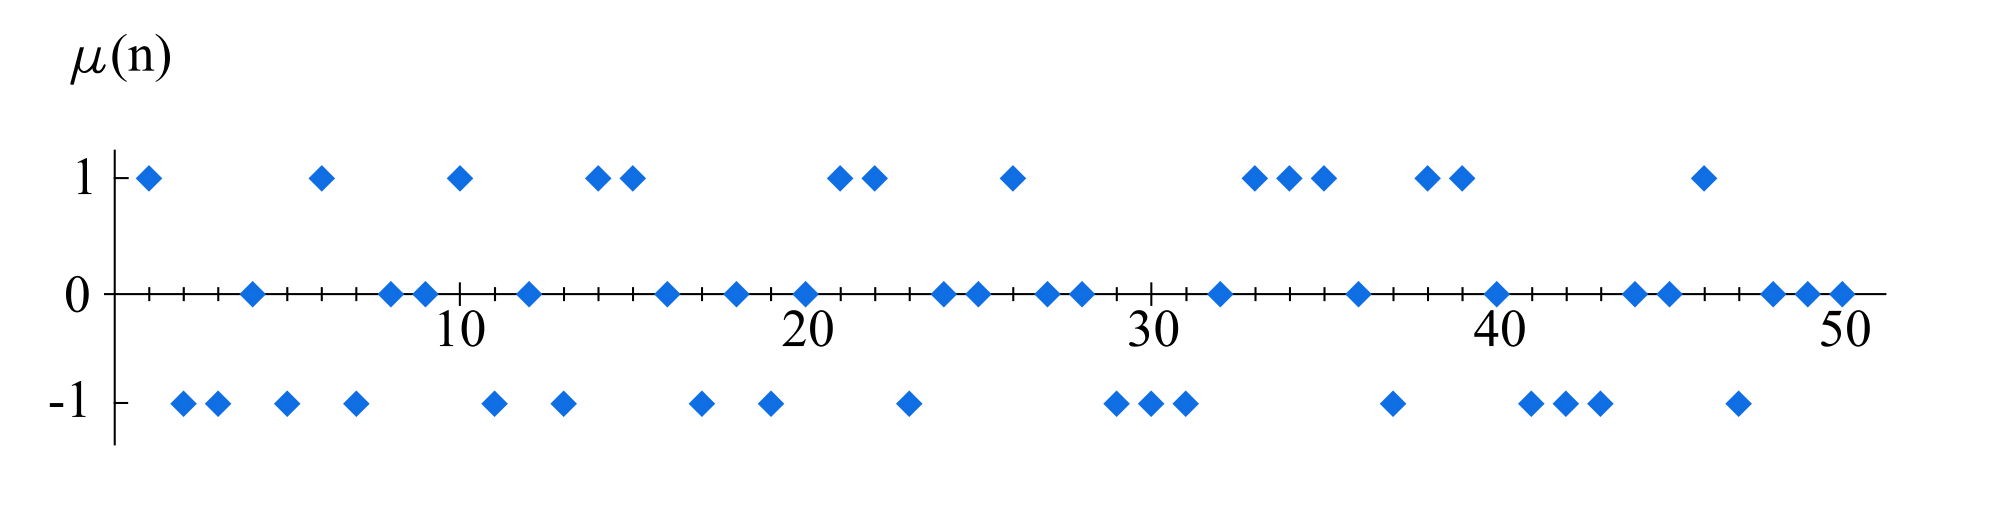
\includegraphics{Moebius_mu.png}
  \caption{First values of the Möbius function $\mu$.}
  \label{fig:MobiusMu}
\end{figure}

\section{Injections, surjections, bijections}

\section{Story time: ``Je le vois, mais je ne crois pas''}

\section{Development: Bendixon-Bernstein-Borel-Cantor-Dedekind-Schröder-Zermelo theorem}

\blindtext

\chapter{Limits and continuity of functions}

\section{Bolzano's theorem}

\blindtext

\section{Story time: the origins of rigorous Calculus}
Stories of this type are best summerized in \href{https://www.smbc-comics.com/comic/how-math-works}{SMBC}.\sidenote{SMBC=Saturday Morning Breakfast Cereal. Similar comics: \href{https://xkcd.com}{xkcd}, \href{http://phdcomics.com}{phdcomics}, \href{https://abstrusegoose.com}{abstruse goose}.}

\section{Development: uniform continuity}

\pagelayout{wide} % No margins
\addpart{[Week V\&VI]\\What are\dots derivatives?}
\pagelayout{margin} % Restore margins

\chapter{Calculations of derivatives}

\section{Formulas}

\section{Monotone functions}

\section{Story time: many-to-one}

\section{Development: Newton quotient}

\chapter{Differentiation: rigorous definition}

\blindtext

\section{Rolle's theorem}

\section{Story time: the Weierstrass function}

\section{Development: Hölder continuity}

\chapter{The main value theorem}

\section{The main value theorem}

\section{The main value inequality}

\section{Story time: Gradient descent}

\section{Development: Sterling's formula}

\pagelayout{wide} % No margins
\addpart{[Week VII\&Beyond]\\Elementary functions and inequalities}
\pagelayout{margin} % Restore margins

\chapter{Exponential function}

\chapter{Logarithm}

\chapter{Trigonometric functions}

\chapter{Hyperbolic functions}

\chapter{Polynomials}

\chapter{Some classical inequalities}

\appendix % From here onwards, chapters are numbered with letters, as is the appendix convention

\pagelayout{wide} % No margins
\addpart{Appendix}
\pagelayout{margin} % Restore margins

\setchapterpreamble[u]{\margintoc}
\chapter{Some more exercises}

\section{Root of unity}\label{Extra:RootUnity}

\section{Constant-recursive sequence}\label{Extra:RecursiveSequence}

\dots

%----------------------------------------------------------------------------------------

\backmatter % Denotes the end of the main document content
\setchapterstyle{plain} % Output plain chapters from this point onwards

%----------------------------------------------------------------------------------------
%	BIBLIOGRAPHY
%----------------------------------------------------------------------------------------

% The bibliography needs to be compiled with biber using your LaTeX editor, or on the command line with 'biber main' from the template directory

% \defbibnote{bibnote}{Here are the references in citation order.\par\bigskip} % Prepend this text to the bibliography
% \printbibliography[heading=bibintoc, title=Bibliography, prenote=bibnote] % Add the bibliography heading to the ToC, set the title of the bibliography and output the bibliography note

%----------------------------------------------------------------------------------------
%	NOMENCLATURE
%----------------------------------------------------------------------------------------

% The nomenclature needs to be compiled on the command line with 'makeindex main.nlo -s nomencl.ist -o main.nls' from the template directory

\nomenclature{$c$}{Speed of light in a vacuum inertial frame}
\nomenclature{$h$}{Planck constant}

\renewcommand{\nomname}{Notation} % Rename the default 'Nomenclature'
\renewcommand{\nompreamble}{The next list describes several symbols that will be later used within the body of the document.} % Prepend this text to the nomenclature

\printnomenclature % Output the nomenclature

%----------------------------------------------------------------------------------------
%	GREEK ALPHABET
% 	Originally from https://gitlab.com/jim.hefferon/linear-algebra
%----------------------------------------------------------------------------------------

\vspace{1cm}

{\usekomafont{chapter}Greek Letters with Pronounciation} \\[2ex]
\begin{center}
	\newcommand{\pronounced}[1]{\hspace*{.2em}\small\textit{#1}}
	\begin{tabular}{l l @{\hspace*{3em}} l l}
		\toprule
		Character & Name & Character & Name \\ 
		\midrule
		$\alpha$ & alpha \pronounced{AL-fuh} & $\nu$ & nu \pronounced{NEW} \\
		$\beta$ & beta \pronounced{BAY-tuh} & $\xi$, $\Xi$ & xi \pronounced{KSIGH} \\ 
		$\gamma$, $\Gamma$ & gamma \pronounced{GAM-muh} & o & omicron \pronounced{OM-uh-CRON} \\
		$\delta$, $\Delta$ & delta \pronounced{DEL-tuh} & $\pi$, $\Pi$ & pi \pronounced{PIE} \\
		$\epsilon$ & epsilon \pronounced{EP-suh-lon} & $\rho$ & rho \pronounced{ROW} \\
		$\zeta$ & zeta \pronounced{ZAY-tuh} & $\sigma$, $\Sigma$ & sigma \pronounced{SIG-muh} \\
		$\eta$ & eta \pronounced{AY-tuh} & $\tau$ & tau \pronounced{TOW (as in cow)} \\
		$\theta$, $\Theta$ & theta \pronounced{THAY-tuh} & $\upsilon$, $\Upsilon$ & upsilon \pronounced{OOP-suh-LON} \\
		$\iota$ & iota \pronounced{eye-OH-tuh} & $\phi$, $\Phi$ & phi \pronounced{FEE, or FI (as in hi)} \\
		$\kappa$ & kappa \pronounced{KAP-uh} & $\chi$ & chi \pronounced{KI (as in hi)} \\
		$\lambda$, $\Lambda$ & lambda \pronounced{LAM-duh} & $\psi$, $\Psi$ & psi \pronounced{SIGH, or PSIGH} \\
		$\mu$ & mu \pronounced{MEW} & $\omega$, $\Omega$ & omega \pronounced{oh-MAY-guh} \\
		\bottomrule
	\end{tabular} \\[1.5ex]
	Capitals shown are the ones that differ from Roman capitals.
\end{center}

%----------------------------------------------------------------------------------------
%	GLOSSARY
%----------------------------------------------------------------------------------------

% The glossary needs to be compiled on the command line with 'makeglossaries main' from the template directory

\newglossaryentry{computer}{
	name=computer,
	description={is a programmable machine that receives input, stores and manipulates data, and provides output in a useful format}
}

% Glossary entries (used in text with e.g. \acrfull{fpsLabel} or \acrshort{fpsLabel})
\newacronym[longplural={Frames per Second}]{fpsLabel}{FPS}{Frame per Second}
\newacronym[longplural={Tables of Contents}]{tocLabel}{TOC}{Table of Contents}

\setglossarystyle{listgroup} % Set the style of the glossary (see https://en.wikibooks.org/wiki/LaTeX/Glossary for a reference)
\printglossary[title=Special Terms, toctitle=List of Terms] % Output the glossary, 'title' is the chapter heading for the glossary, toctitle is the table of contents heading

%----------------------------------------------------------------------------------------
%	INDEX
%----------------------------------------------------------------------------------------

% The index needs to be compiled on the command line with 'makeindex main' from the template directory

\printindex % Output the index

%----------------------------------------------------------------------------------------
%	BACK COVER
%----------------------------------------------------------------------------------------

% If you have a PDF/image file that you want to use as a back cover, uncomment the following lines

%\clearpage
%\thispagestyle{empty}
%\null%
%\clearpage
%\includepdf{cover-back.pdf}

%----------------------------------------------------------------------------------------

\end{document}
